\documentclass{if-beamer}

% --------------------------------------------------- %
%                  Presentation info	              %
% --------------------------------------------------- %
\title[Modulador]{Modulador Para El amplificador clase D}
\subtitle{Universidad ICESI}
\author{M. Gallego. R, \\
N. J. Salazar. E.}
\institute[ICESI]{
}
\date{\today}
\logo{

\includegraphics[scale=0.080]{figuras/ICESI.jpeg}
}
\subject{Presentation subject} % metadata

\graphicspath{{figuras/}}
% --------------------------------------------------- %
%                    Title + Schedule                 %
% --------------------------------------------------- %

\begin{document}

\begin{frame}
  \titlepage
\end{frame}

\begin{frame}{Contenido}
  \tableofcontents
\end{frame}

% --------------------------------------------------- %
%                      Presentation                   %
% --------------------------------------------------- %
%%%%%%%%%%%%%%%%%%%%%%%%%%%%%%%%%%%%%%%%%%%%%%%%%%%%%%%
%%%%%%%%%%%%%%%%%%%%%%%INTRODUCCCIÓN%%%%%%%%%%%%%%%%%%%
%%%%%%%%%%%%%%%%%%%%%%%%%%%%%%%%%%%%%%%%%%%%%%%%%%%%%%%
\section{Introducción}
\subsection{¿Qué es una modulación?}
\begin{frame}{¿Qué es una modulación?}

Es la modificación de un parametro de la señal por otra, este 
párametro puede ser frecuencia, amplitud, fase, los elementos que hacen parte de la modulación son: 

\begin{itemize}
    \item \textbf{señal portadora: } Es la señal encargada de transportar la información su frecuencia es la frecuencia de transmisión 
    \item \textbf{Señal moduladora: } Es la señal que contiene la información 
    \item \textbf{Señal modulada: } Es la señal que resulta de la modulación 
\end{itemize}{}
\end{frame}{}

%%figura modulación 
\begin{frame}{}
\begin{figure}[h]
\setlength{\unitlength}{0.14in}
\centering
\begin{picture}(32,15)
\put(12,6){\framebox(6,3){$Modulator$}}
\put(8,7.5){\vector(1,0){4}}
\put(8,7.6){ $ input $ }
\put(18,7.5){\vector(1,0){4}}
\put(19,7.6){ $ output $ }
\put(5,7.5){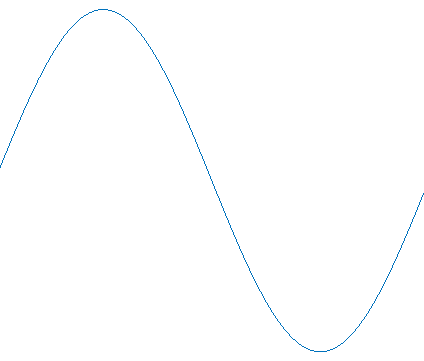
\includegraphics[scale=0.090]{figuras/sin.png}}
\end{picture}
\caption{proceso de modulación} % title of the Figure
\label{fig:1}
 % label to refer figure in text
\end{figure}
\end{frame}

\subsection{¿Qué es el muestreo?}
\begin{frame}{¿Qué es el muestreo?}
\begin{center}
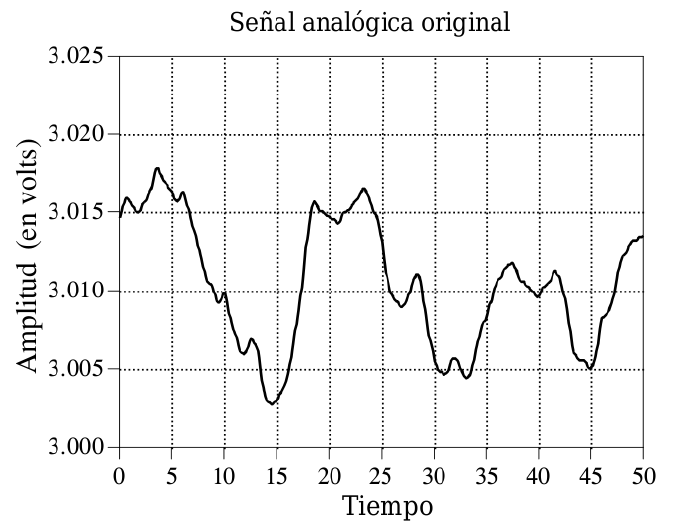
\includegraphics[scale=0.40]{figuras/senal.png}
\end{center}{}
\end{frame}{}

\begin{frame}{}
\begin{center}
    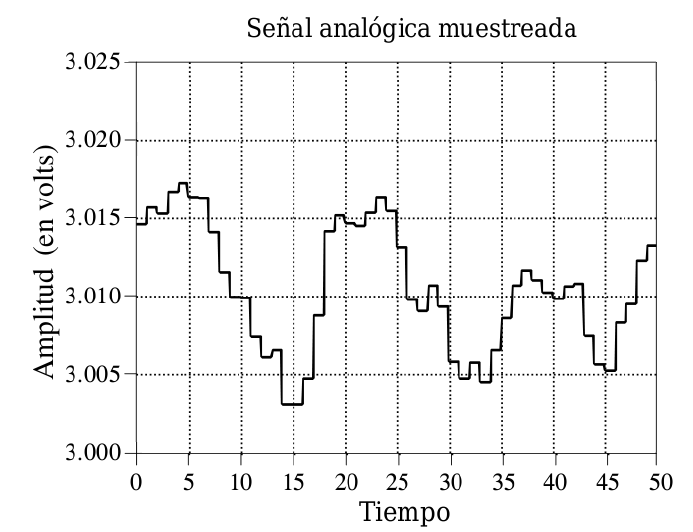
\includegraphics[scale=0.4]{figuras/senal2.png}
\end{center}{}
    
\end{frame}{}

\subsection{Modulación PWM}
\begin{frame}{Modulación PWM (modulación por duración de pulso)}
    Modulación por duración de pulso 
    
    \begin{center}
        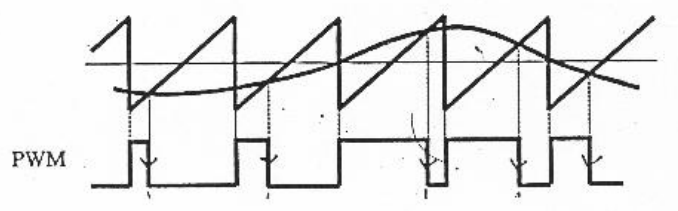
\includegraphics[scale=0.4]{figuras/pulso.png}
    \end{center}{}
    
\end{frame}{}
%%%%%%%%%%%%%%%%%%%%%%%%%%%%%%%%%%%%%%%%%%%%%%%%%%%%%%%
%%%%%%%%%%%%%%%%%%%%%%IMPLEMENTACIÓN%%%%%%%%%%%%%%%%%%%
%%%%%%%%%%%%%%%%%%%%%%%%%%%%%%%%%%%%%%%%%%%%%%%%%%%%%%%
\section{Implementación del Modulador}

\subsection{Materiales}
\begin{frame}{Materiales}
\end{frame}{}

\subsection{Montaje}
\begin{frame}{Montaje}
\end{frame}{}

\subsection{Resultados}
\begin{frame}{Resulatdos}
\end{frame}{}

\section{Conclusiones}
\begin{frame}{Conclusiones}
\end{frame}{}

\end{document}
